\section{Supplementary material}

\subsection{Outcome modelling}

We derived each mRS distribution for treatment at \emph{t=0} using the methodology of log-odds ratio of a good outcome falling linearly with time to treatment \cite{emberson_effect_2014, fransen_time_2016}. For each of the nLVO and LVO mRS distributions, we use the change of log-odds ratio of mRS 0-1 with time to IVT \cite{emberson_effect_2014} to scale the probability of mRS 0-1 from \emph{t=No Effect} to \emph{t=0}. We also require the mRS distributions for each patient cohort pre-stroke (sourced from SSNAP data) and if they received no treatment. The nLVO no-treatment population is the weighted difference of no-treatment populations containing both patients with nLVOs and LVOs \cite{lees_time_2010} and containing only LVO patients \cite{goyal_endovascular_2016}, where weights of 149\% and 49\% respectively result in the nLVO no-treatment probability of mRS 0-1 matching a reference population \cite{emberson_effect_2014}. The resulting proportions of LVO (49\%) and nLVO (51\%) patients are similar to those in clinical trials \cite{ist-3_collaborative_group_benefits_2012, emberson_effect_2014}. 
These \emph{t=0} mRS 0-1 data inform the weights for weighted averages of the pre-stroke and \emph{t=No Effect} mRS distributions that create the full \emph{t=0} mRS distributions (64.3\% and 35.7\% for nLVO, 25.5\% and 74.5\% for LVO respectively). The resulting \emph{t=No Effect} and \emph{t=0} mRS distributions for nLVO are consistent with the decline of chance of mRS 0-1 with time \cite{holodinsky_modeling_2018}. The MT \emph{t=0} mRS distribution is defined as the weighted average of 75\% of the pre-stroke and 25\% of the \emph{t=No Effect} distributions, following a reference rate of successful recanalisation \cite{hui_efficacy_2020}. The MT excess death rate is set to 4.0\% to ensure that log-odds falling linearly with time between the values of mRS 0-5 in the \emph{t=0} and in the \emph{t=No Effect} mRS distributions is consistent with a reference average mortality rate at the average MT time \cite{goyal_endovascular_2016}. The resulting \emph{t=0} and \emph{t=No Effect} mRS 0-2 probabilities give close matches to a reference decline of chance of mRS 0-2 with time \cite{fransen_time_2016}.

The time to no effect was 6.3 hours for IVT \cite{emberson_effect_2014} and 8.0 hours for MT \cite{ fransen_time_2016} (our model did not include selection of patients who may still benefit from treatment beyond these durations). We derived each \textit{No Effect} mRS distribution by applying the excess death rate due to treatment equally across the patient’s mRS distribution had they not received treatment (to represent that no benefit from treatment has been received as it was given too late, but the patient has been exposed to the risk from receiving the treatment).

We calculate the remaining IVT data using excess death rates of 1.1\% for nLVO and 3.4\% for LVO, from the difference in death rates of trial groups given IVT and given no treatment \cite{emberson_effect_2014}.

\subsection{Zoom in on benefit around one CSC (MSU base location)}

Figure \ref{fig:map_zoom} shows details of area of benefit/disbenfit of using MSU care over usual care. There is a halo of maximum benefit further out from the CSC where patients avoid an inter-hospital transfer (and associated delays for MT), but this enhanced benefit erodes with further travel time for the MSU.

\begin{figure}[h!]
    \centering
    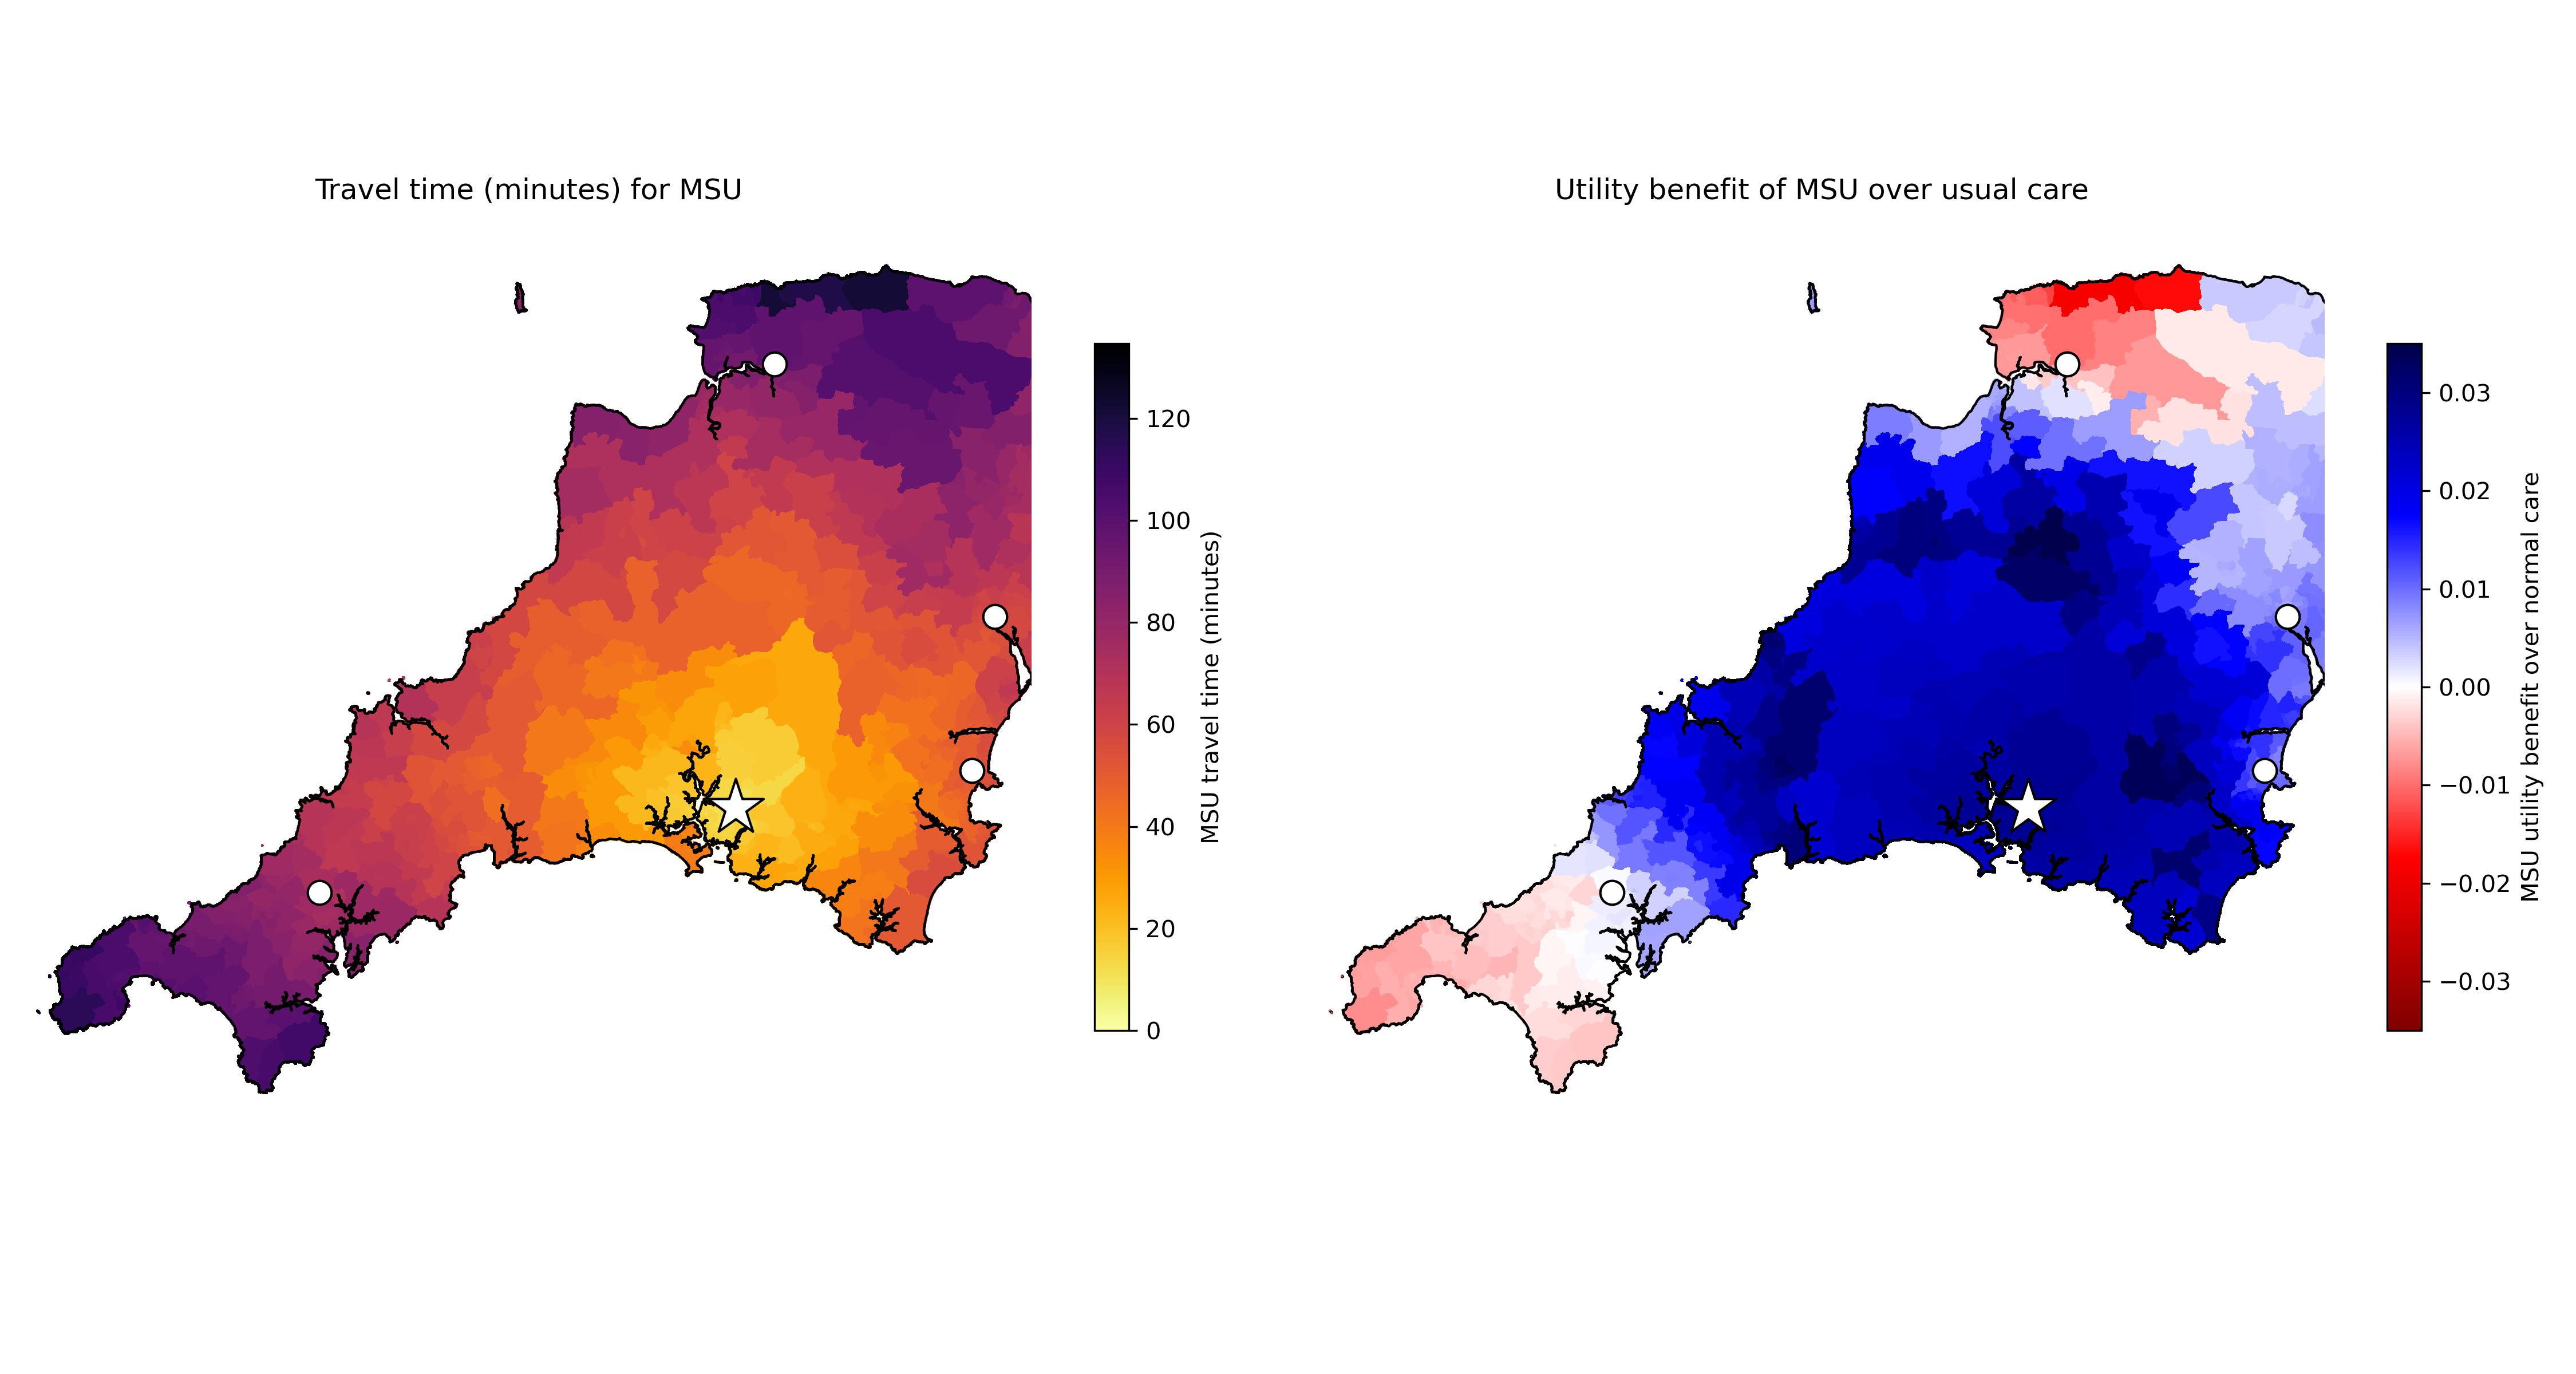
\includegraphics[width=1.0\linewidth]{images/map_zoom.jpg}
    \caption{Travel time for the MSU (to patient, and return travel for MT) and the utility benefit of using MSU care over usual care.}
    \label{fig:map_zoom}
\end{figure}

\subsection{Top 10 locations for MSUs}

Figure \ref{fig:top_10} shows the first 10 locations chosen by a greedy algorithm, where MSU locations are added one at a time, with each new location selected based on the best possible improvement in utility by adding one more unit.

\begin{figure}[h!]
    \centering
    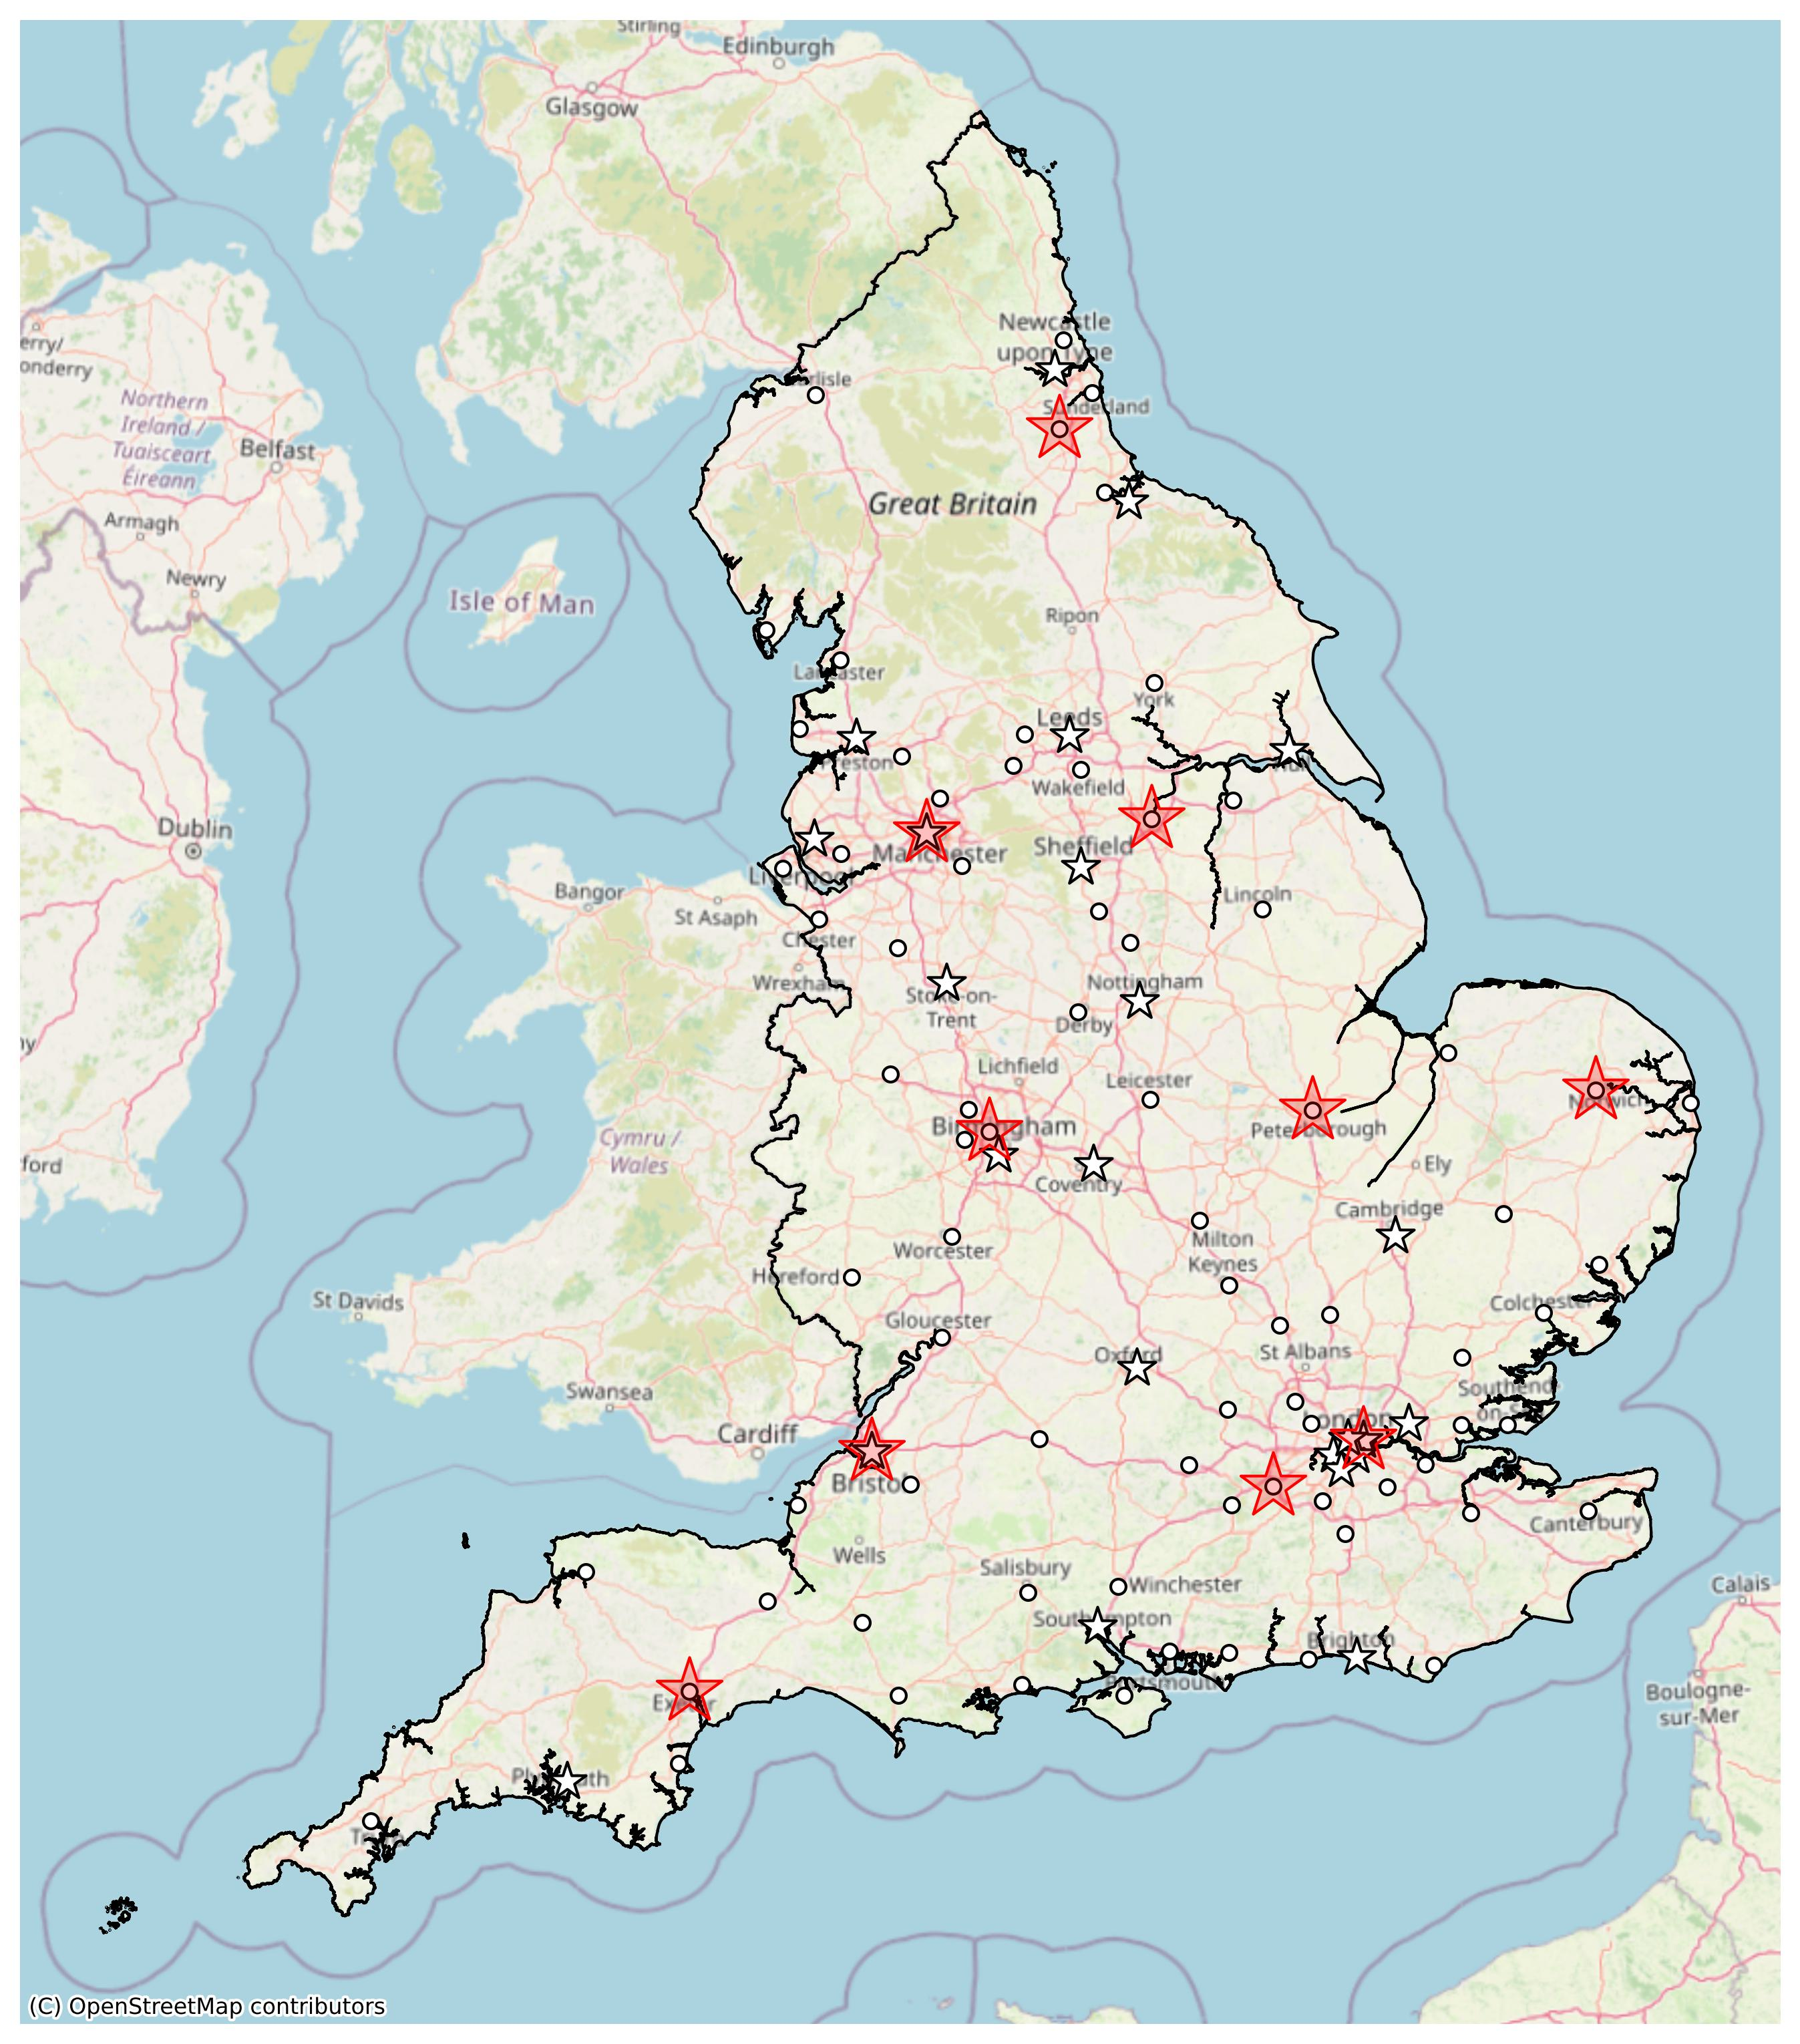
\includegraphics[width=1.0\linewidth]{images/top_10_msu_map.jpg}
    \caption{Top 10 locations (red stars) chosen by a greedy algorithm for maximising benefit from MSUs. White circles show locations of PSCs (providing only IVT). White stars show locations of CSCs.}
    \label{fig:top_10}
\end{figure}